\section{Définition}
Les shaders sont des programmes plus ou moins élaborés qui ne sont pas pris en charge par le CPU (processeur), mais par le GPU (carte graphique). Exécutés sur chaque primitive d’une forme, ils permettent un affichage calculé, de pixels en couleur pour un rendu graphique. Les paramètres de ces couleurs sont : la teinte, la luminance, la saturation.
\section{Historique}
Du point de vue des bibliothèques graphiques, les shaders ont été intégrés à partir d'OpenGL 2.0 et dans DirectX 8.
\\
Pour chaque version différente de shader, nous parlons de modèles de shader (shader models (SM)). Il est possible de préciser la version que nous voulons utiliser dans notre shader.

\begin{center}
\begin{tabular}{|c|c|c|c|m{0.1\linewidth}|m{0.1\linewidth}|}
\hline
Année & Version	& DirectX & OpenGL & ATI & Nvidia\\
\hline
2001 & SM 1.x & DirectX8 & OpenGL 2.0 & Radeon R200 & Geforce séries 3\\
\hline
2003 & SM 2.x & DirectX9.0 & & Radeon R300 / R420 & Geforce FX\\
\hline
2004 & SM 3.0 & DirectX9.0c & & Radeon R520	& Geforce séries 6 / 7\\
\hline
2006 & SM 4.0 & DirectX10 & OpenGL 3.2 & Radeon R600 & Geforce séries 200 / 300\\
\hline
2009 & SM 5.0 & DirectX11 & OpenGL 4.1 & Radeon R800 & Geforce séries 400\\
\hline
\end{tabular}
\end{center}

\section{Fonctionnement}
\subsection{Vertex Shader}
Le vertex shader est exécuté pour chaque vertex (sommet).
\\\\
Il remplace la tâche dite de Transform \& lighting. Elle doit dans un premier temps calculer la projection de coordonnées des sommets à partir de l'espace 3D dans l'espace écran et dans un second temps, définir l’éclairage pour chaque sommet.
\\\\
La projection des formes est le plus souvent décomposée en triangles, car les triangles permettent en remplissage des surfaces complexes sans pertes.
\\\\
Le vertex shader reçoit en entrée un sommet, un ensemble  de paramètres constants.
\\\\
Le vertex shader renvoie en sortie le même sommet qu’en entrée, mais transformé, avec des attributs spéciaux comme ses coordonnées dans l’espace écran (obligatoire), et des attributs interpolés comme la couleur (obligatoire), la texture (facultatif)…
\\\\\\
Possibilités du vertex shaders :
\begin{itemize}
  \item Position procédurale
  \item Mélange de transformations (‘Vertex Blend’)
  \item Mélange de maillages (‘Morphing’) 
  \item Déformation du maillage (‘Vertex Deformation’)
  \item Eclairage par sommet (‘Per Vertex Lighting’)
  \item Tissu, peau, interpolation, displacement maps…
  \item Coordonnées de texture
  \item Brouillard particulier
  \item Taille d’affichage d’un point
  
\end{itemize} 

\textbf{\\Transform} est la tâche qui permet de convertir des données spatiales depuis un espace virtuel en 3D vers l'écran en 2D.
\\\\
\textbf{Lighting} est la 3e opération qui va permettre d'éclairer la scène : éclairage des objets dans la scène 3D, calcul de l'intéraction des composantes de la lumière sur les objets puis envoi de la scène ainsi calculée à l'écran.
\\\\
\textbf{Architecture} :
\\
\begin{center}
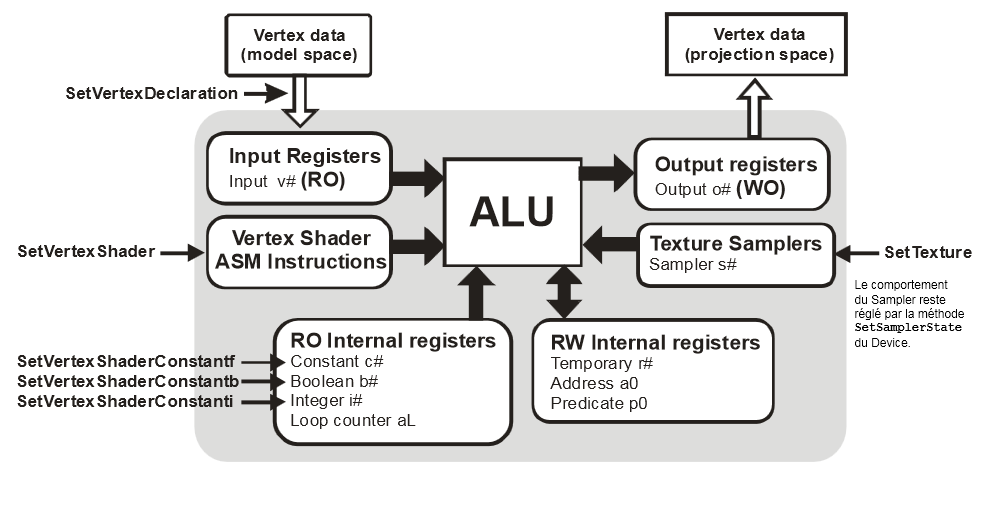
\includegraphics[width=12cm,height=60mm]{pipeline/images/ArchiVertex.png}
\end{center}

\textbf{ALU} (Arithmetic logic unit) : C’est l’unité qui effectue les calculs, grâce aux variables contenues dans les registres.
\\\\
Description des registres de la structure :

\subsection{Fragment Shader}
Un fragment est un pixel qui n’a pas encore été traité. Ses attributs sont définis par le vertex shader, et interpolés par la rastérisation.
Le fragment shader ou pixel shader est exécuté pour chaque pixel de la forme délimitée par les vertex. Il remplace la tâche dite de "multitexturing". Son rôle étant de définir la couleur ou la texture de chaque pixel en fonction des couleurs, de l’éclairage et de la profondeur de chaque vertex de la forme.
Le fragment shader reçoit en entrée un fragment et ses attributs résultant de l’interpolation des sommets comme sa couleur, ses coordonnées.
Le fragment shader renvoi en sortie le fragment d’entrée transformé en pixel, avec sa profondeur, sa couleur, sa transparence, ou aucun pixel (suppression de pixel).
Possibilités du fragment shaders :
\begin{itemize}
	\item Réflexion par pixel
	\item Illumination par pixel (phong, BRDF) -> plus de dégradé
	\item Textures procédurales
	\item Cartoon shading
	\item nouveaux modèles d’ombrages (par pixel, géométrie interpolée).
	\item textures procédurales ou dynamiques.
	\item bump-mapping
\end{itemize}
\textbf{Architecture} :
\\
\begin{center}
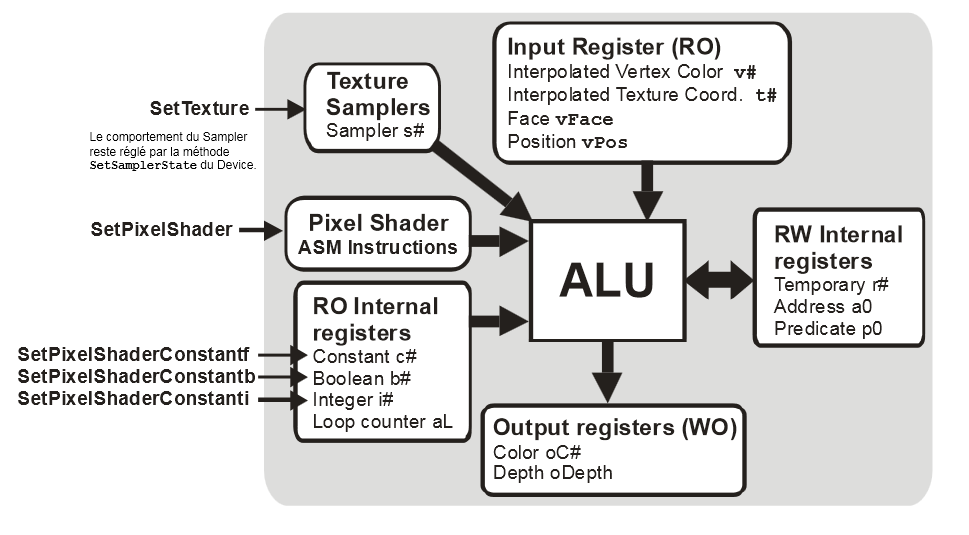
\includegraphics[width=12cm,height=60mm]{pipeline/images/ArchiPixel.png}
\end{center}

\subsection{Geometry Shader}
Créer de nouvelles formes géométriques.
\\

\section{Langages}
Les GPUs peuvent être programmés grâce au langage dit « Shading language ». C’est un langage de description des interactions simples ou complexes, entre la lumière et la matière.\\
\textbf{\\GLSL} (OpenGL Shading Language) : 
\begin{itemize}
	\item Intégré à OpenGL.
	\item Plus simple que Cg.
	\item OpenGL se charge d’inclure les shaders.
	\item Multi-platforme (IOS, Windows, Android…).
	\item Exclusif à OpenGL.
	\item Peu d’outils additionnels.
	\item Support moindre que HLSL ou Cg.
\end{itemize}
\textbf{\\HSLS} :
\begin{itemize}
	\item Se charge d’inclure les shaders.
\end{itemize}
\textbf{\\Cg} (C for graphics) : 
\begin{itemize}
	\item Indépendant de l’API 3d (Direct3D ou OpenGL).
	\item Outil débogueur
	\item Le plus utilisé
	\item Support important
	\item Windows uniquement
\end{itemize}
\begin{center}
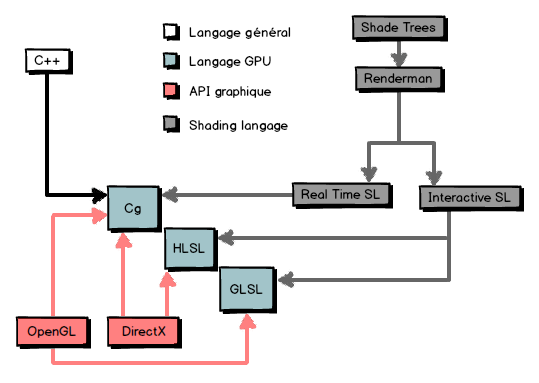
\includegraphics[width=14cm,height=100mm]{pipeline/images/langages.png}
\end{center}